\documentclass[onecolumn, draftclsnofoot,10pt, compsoc]{IEEEtran}
\usepackage{graphicx}
\usepackage{url}
\usepackage{setspace}

\usepackage{listings}
\usepackage{xcolor}
\usepackage{float}

\usepackage{geometry}
\geometry{textheight=9.5in, textwidth=7in}

\usepackage{hyperref}
\hypersetup{
    colorlinks=true,
    linkcolor=blue,
    filecolor=magenta,      
    urlcolor=cyan,
}

\makeatletter
\renewcommand\paragraph{\@startsection{paragraph}{4}{\z@}%
            {-2.5ex\@plus -1ex \@minus -.25ex}%
            {1.25ex \@plus .25ex}%
            {\normalfont\normalsize\bfseries}}
\makeatother
\setcounter{secnumdepth}{4} % how many sectioning levels to assign numbers to
\setcounter{tocdepth}{4}    % how many sectioning levels to show in ToC


\definecolor{lightgray}{rgb}{.9,.9,.9}
\definecolor{darkgray}{rgb}{.4,.4,.4}
\definecolor{purple}{rgb}{0.65, 0.12, 0.82}

\lstdefinelanguage{JavaScript}{
  keywords={typeof, new, true, false, catch, function, return, null, catch, switch, var, if, in, while, do, else, case, break},
  keywordstyle=\color{blue}\bfseries,
  ndkeywords={class, export, boolean, throw, implements, import, this},
  ndkeywordstyle=\color{darkgray}\bfseries,
  identifierstyle=\color{black},
  sensitive=false,
  comment=[l]{//},
  morecomment=[s]{/*}{*/},
  commentstyle=\color{purple}\ttfamily,
  stringstyle=\color{red}\ttfamily,
  morestring=[b]',
  morestring=[b]"
}
 
\urlstyle{same}

% 1. Fill in these details
\def \CapstoneTeamName{		ConnectBasket Development Team}
\def \CapstoneTeamNumber{		39}
\def \GroupMemberOne{			Henry Fowler}
\def \GroupMemberTwo{			Kailyn Hellwege}
\def \GroupMemberThree{			Taylor Kirkpatrick}
\def \CapstoneProjectName{		ConnectBasket}
\def \CapstoneSponsorCompany{	OSU MIME}
\def \CapstoneSponsorPerson{		Dr. Chinweike Eseonu}

% 2. Uncomment the appropriate line below so that the document type works
\def \DocType{		%Problem Statement
				%Requirements Document
				%Technology Review
				%Design Document
				Final Report
				}
			
\newcommand{\NameSigPair}[1]{\par
\makebox[2.75in][r]{#1} \hfil 	\makebox[3.25in]{\makebox[2.25in]{\hrulefill} \hfill		\makebox[.75in]{\hrulefill}}
\par\vspace{-12pt} \textit{\tiny\noindent
\makebox[2.75in]{} \hfil		\makebox[3.25in]{\makebox[2.25in][r]{Signature} \hfill	\makebox[.75in][r]{Date}}}}
% 3. If the document is not to be signed, uncomment the RENEWcommand below
\renewcommand{\NameSigPair}[1]{#1}

%%%%%%%%%%%%%%%%%%%%%%%%%%%%%%%%%%%%%%%
\begin{document}
\begin{titlepage}
    \pagenumbering{gobble}
    \begin{singlespace}
    	
\includegraphics[height=4cm]{coe_v_spot1}
        \hfill 
        % 4. If you have a logo, use this includegraphics command to put it on the coversheet.
        %\includegraphics[height=4cm]{CompanyLogo}   
        \par\vspace{.2in}
        \centering
        \scshape{
            \huge CS Capstone \DocType \par
            {\large\today}\par
            \vspace{.5in}
            \textbf{\Huge\CapstoneProjectName}\par
            \vfill
            {\large Prepared for}\par
            \Huge \CapstoneSponsorCompany\par
            \vspace{5pt}
            {\Large\NameSigPair{\CapstoneSponsorPerson}\par}
            {\large Prepared by }\par
            Group\CapstoneTeamNumber\par
            % 5. comment out the line below this one if you do not wish to name your team
            \CapstoneTeamName\par 
            \vspace{5pt}
            {\Large
                \NameSigPair{\GroupMemberOne}\par
                \NameSigPair{\GroupMemberTwo}\par
                \NameSigPair{\GroupMemberThree}\par
            }
            \vspace{20pt}
        }
        \begin{abstract}
        % 6. Fill in your abstract    
        This document gives a detailed description of the ConnectBasket project. All requirements and the design of the project will be given as well as any changes that ended up being made during development of the project. The decisions for what technologies to use for the project will also be given along with important documents related to the project such as the poster and instructional documentation.

        \end{abstract}     
    \end{singlespace}
\end{titlepage}
\newpage
\pagenumbering{arabic}
\tableofcontents
% 7. uncomment this (if applicable). Consider adding a page break.
%\listoffigures
%\listoftables
\clearpage

% 8. now you write!

\section{Introduction to Project}

\subsection{Project Purpose}
This project will create a web application called ConnectBasket that will serve as a new tool for the Oregon State University Veterinary Hospital to improve communication within the hospital and externally with patient owners and other hospitals. The current workflow in the hospital involves receptionists taking calls, typing a message into the system, printing out that message, and walking it across the hospital to a veterinary technician or doctor to look at and add a handwritten note to. After that, the doctor or technician will carry the message to another doctor or technician, or back to reception or scheduling, who will call the initial caller and answer the question they had or schedule an appointment for them. The main purpose of this project is to eliminate the paper aspects of this process and make an electronic system that allows messages to be created and sent to other employees of the hospital, and notes to be added to those messages. It will then be able to display messages back to users with all of their associated notes. This project will help increase the efficiency of communication at the hospital as well as provide a less error-prone system that allows users to see a complete history of all messages.

\subsection{Project Goals}
\begin{itemize}
\item Allow users to create a message which will be associated with a patient and an owner of that patient
\item Allow messages to have a status to tell whether they are open or closed
\item Allow messages to be routed to other users or groups of users
\item Allow notes to be added to messages
\item Allow users to select a group or groups to be a part of
\item Provide an audit log of all messages created over a given time period
\item Increase the overall efficiency of messages being transported throughout the hospital 
\item Reduce the amount of paper being printed
\item Reduce errors in the communication process of the hospital 
\end{itemize}

\subsection{Clients}
The official client was Dr. Chinweike Eseonu, a professor in the College of Engineering at Oregon State University. The other client was Kelly Warner, the Process Improvement Manager at the Oregon State University Veterinary Hospital.

\subsection{Development Team}
All parts of the project were discussed and planned by all members of the team, but each team member had specific parts of the project they focused on. Most features of the website were a result of contribution from multiple team members.

\subsubsection {Henry Fowler}
Henry focused on the database and back end of the project. Designing and creating the tables and stored procedures stored in the MySQL database and writing the PHP code to interact with the database from the website.

\subsubsection {Kailyn Hellwege}
Kailyn was responsible for most of the front end development of the website. Writing the HTML and CSS that style all of the pages of the site and the Javascript code that makes the pages dynamic.

\subsubsection {Taylor Kirkpatrick}
Taylor designed and created the notification system for the website, including the shell script responsible for sending the notifications. He also worked on setup and configuration of the web server that the website is running on.

\subsection{Role of the Clients}
Dr. Eseonu provided some guidance and suggestions about overall design and features of the project. Kelly provided most of the input into what the website should look like and what features were needed.

\newpage
\section{Requirements Document}
\subsection{Introduction}

\subsubsection{Purpose}
The purpose of this document is to outline the requirements for an improved communication system for the Oregon State University (OSU) Veterinary Hospital, called ConnectBasket. 
This document's audience is the client, as well as certain staff members at the hospital. This document will be used as a way to measure the success of the Capstone development team working on this project. 


\subsubsection{Scope}
ConnectBasket will be a web based portal for the OSU Veterinary Hospital that will streamline the way messages are moved around the hospital and provide a better way to track the route that messages have taken. When an owner calls the hospital, receptionists will be able to type a message into the computer, assign it a category, and route it to the necessary staff members, which may be service specific vet techs, house officers, or faculty. Those staff members will be alerted, either by email or text, that they have a message waiting for them in ConnectBasket, and once viewed, notes can be added and the message can be re-routed to other staff members. After a message has been addressed by the necessary staff, the message can be closed, meaning no more notes can be added. The audit trail of when the message was created and closed will be visible, along with all the notes, timestamps of notes, and staff who added the notes.


\subsubsection{Definitions, Acronyms, and Abbreviations}
\begin{itemize}
\item Capstone - CS 461 class at Oregon State that the developers of ConnectBasket are in
 
\item OSU - Oregon State University

\item Hospital - referring to the OSU Veterinary Hospital

\item Owner - a person who owns a pet that is a client of the hospital

\item Patient - an animal who has/is going to be treated at the hospital 

\item VetHosp - the hospital management system used by the OSU Veterinary Hospital for keeping patient and owner records

\item Mobile Devices - smartphones or tablets
\end{itemize}
\subsubsection{References}
IEEE Std 830-1998, IEEE Recommended Practice for Software Requirements Specifications

\subsubsection{Overview}
The second section of this document will contain a further description of the ConnectBasket project, including product functions, user characteristics, and constraints. The third section will define the specific requirements of the project. 

\subsection{Overall Description}

\subsubsection{Product Perspective}
The ConnectBasket web based portal will be a stand alone system that will have additional functionality to connect to the current VetHosp system used by the hospital. ConnectBasket will use patient and owner information stored in the VetHosp system to connect information collected with the correct patients and owners, given that access to the data in VetHosp is provided to the Capstone development team.

\paragraph{User Interfaces}
There will need to be some level of security requiring users to login to access the information in the system. The system will provide users with the ability to search for a patient or owner and to enter new messages for them as well as view older messages and the audit trail associated with the message.

\paragraph{Hardware Interfaces}
Staff will be able to access the system from their desktop or laptop computers as well as mobile devices.

\paragraph{Software Interfaces}
ConnectBasket might be able to interface with the VetHosp program in order to connect information collected with the information about patients and owners stored in VetHosp. Access to the patient and owner information stored in VetHosp will be required for a system that could be integrated with VetHosp.

\subsubsection{Product Functions}
\paragraph{User Stories}
The receptionists at the hospital will need to be able to take calls from owners, enter a message into ConnectBasket, and forward it on to necessary staff members, such as vet techs or doctors. After that, the staff receiving the message can perform the action requested of them, and add any notes to the message. Then, it can be rerouted to other staff members. At the end of the chain, the message will be routed back to scheduling or reception, where they can contact the owner with information or to set up an appointment. They will then mark the chain as closed, and it will be able to be viewed later by staff members with permission to view audit logs.
\paragraph{Function Dependencies}
See Original Gantt Chart.

\subsubsection{User Characteristics}
Users of ConnectBasket will be staff members of the hospital. The users will have a variety of different education levels and experience. Therefore, the system will need to be designed so that technical expertise is not required in order to properly use it.

\subsubsection{Constraints}
The performance of the ConnectBasket application will be limited by a staff member's internet connection. Staff should not use the service on unsecure networks, as messages sent with it should have some degree of confidentiality due to the nature of the work, the hospital's policies, and government regulations. This limits where the application can be accessed from, as non-trusted networks may expose these messages. Staff may also only access this application with a verified user account.

\subsubsection{Assumptions and Dependencies}
It will be assumed that staff will not be attempting to use non-English languages for messaging. This system might depend on the hospital's existing VetHosp software, and integration with it is a goal for this project. Integration will depend on the VetHosp software being available to the developers and the level of access the Capstone development team will have to it. VetHosp integration will also depend on the hospital's IT team arranging an integration of ConnectBasket with VetHosp. Any changes that need to be made to the VetHosp system for integration will need to be done by the team in charge of developing VetHosp, not the Capstone development team. However, ConnectBasket will be capable of operating independently without any integration.

\subsection{Specific Requirements}

\subsubsection{External interface requirements}

\paragraph{VetHosp}
ConnectBasket might be integrated with VetHosp as it nears completion, so that it can pull information from VetHosp as needed to populate fields and reduce separate instances of data lookup. Detailed information about VetHosp is not currently available to the development team, and successful integration will depend on the level of access provided to the Capstone development team.

\subsubsection{System features}

\paragraph{Creation of Messages}
ConnectBasket will allow receptionists to create messages and route them to other parts of the hospital. Receptionists and other staff should be able to route messages with patient information to the relevant locations in the hospital. These messages should be secure and not exposed to public channels, and may need to be encrypted as well.

\paragraph{Message Auto Population}
ConnectBasket will allow message composers to easily write messages by auto populating some fields of the message, such as the current date and patient and owner names. By auto filling and not allowing free text for certain fields, message creation will be more efficient and less error-prone. These fields will be prefilled for convenience and to send off messages quicker and in a standard format. This feature will also include utilizing drop-down menus instead of plain text to reduce error for other fields, such as recipients of messages and category of messages.

This feature will be useful for both convenience and safety, as constraining messages to at least some pre-defined standard will reduce the likelihood of human error in medical situations.

\paragraph{Message Notification}
ConnectBasket will send message recipients notifications when a message has been routed to them or a category their profile belongs to. Notifications will be delivered as a text message, email, or both, depending on the preferences of the staff member. Staff members will have the option to receive alerts simply after a message is received or after a message is unread for a portion of time.

\paragraph{Message Review and Forwarding}
ConnectBasket will allow message recipients to review their messages online via any internet-accessible device, should the connection or other factors not restrict them from doing so. Staff who have viewed a message will be capable of rerouting this same message to other necessary staff, along with any comments or addendums added by the previous recipient. 

\paragraph{Message Resolution}
ConnectBasket will allow message recipients to resolve messages as closed, should the task or job mentioned within it be completed. This closed state should remove the message from all staff member's queues, allowing them to focus on other tasks that have not been resolved.
	
Ideally, this feature will include more than just a closed state; it will include additional states that show other reasons for a task to no longer be active, such as cancelled, duplicate, or stopped, to provide more information about the status of a task.

\paragraph{Message Audit Record}
ConnectBasket will allow staff with sufficient permissions to view a message's  history for audit or review. Authorized staff will  be able to see when and where the message was created, when and where it was routed, and when and where it was closed. The name of any staff member who took any action should also be recorded, along with other activity regarding a message. 

Providing an audit trail for all messages will provide the hospital with valuable information and allow them to track metrics such as the average amount of time the hospital takes to respond to calls and common reasons for owners calling the hospital. 

\paragraph{Message Recipient Roles and Profile Roles}
ConnectBasket will allow staff to select and be assigned to one or more roles that reflect their duties and responsibilities at the hospital. Staff will have profiles to manage their roles, with the ability to change their roles at will. When messages are routed to a specific department, any staff member that has selected the associated role to that department will receive the message in a queue accessible by anyone assigned to the role. These staff members will be able to take ownership of the message to interact with it, or interact with it to a lesser degree without taking ownership of the message. All of the regular message features that are accessible to individual staff members will also be accessible to the all the staff members that receive a message in a role. 

Staff in one location can not assume, and should not have to assume, whether a certain employee is available or whether a task falls under their responsibilities. Assigning messages to a role and putting them in queues removes the necessity for staff to understand structure in other departments, and allows tasks and messages to be passed faster and with less room for error.

\subsubsection{Performance Requirements}

\paragraph{Web Service}
This web based portal will need to be accessible from any internet accessible device. Staff will be doing vital work through this application, and so it must be accessible to them, no matter what device they have. However, there are constraints on how accessible this is. Internal messaging must remain confidential and secure, and staff should have secure profiles to restrict access to malicious persons. ConnectBasket must be reliable and have minimal downtime, as this application going down could cripple the work of the hospital staff once it is deployed. Downtime should be kept to a maximum of two hours a week once in a fully completed state. Two hours per week allows for security patching and maintenance should it be required, though this number may change depending on the specific processes as they are defined.

\subsubsection{Design Constraints}
ConnectBasket will be constrained only by any government or hospital regulations on message security or reliability. Regulations may require audit trails or set a maximum downtime for the application, which will restrict the design as these come to light.

In addition, while not a mandatory constraint, eventual integration with VetHosp is the long term goal for this project. If the project is built in such a way as to ease the connection between the two, this design choice may save a significant amount of time. However, with a lack of knowledge about VetHosp, designing in such a way is unlikely and thus, not a mandatory element of the design.

\subsection{Original Gantt Chart}
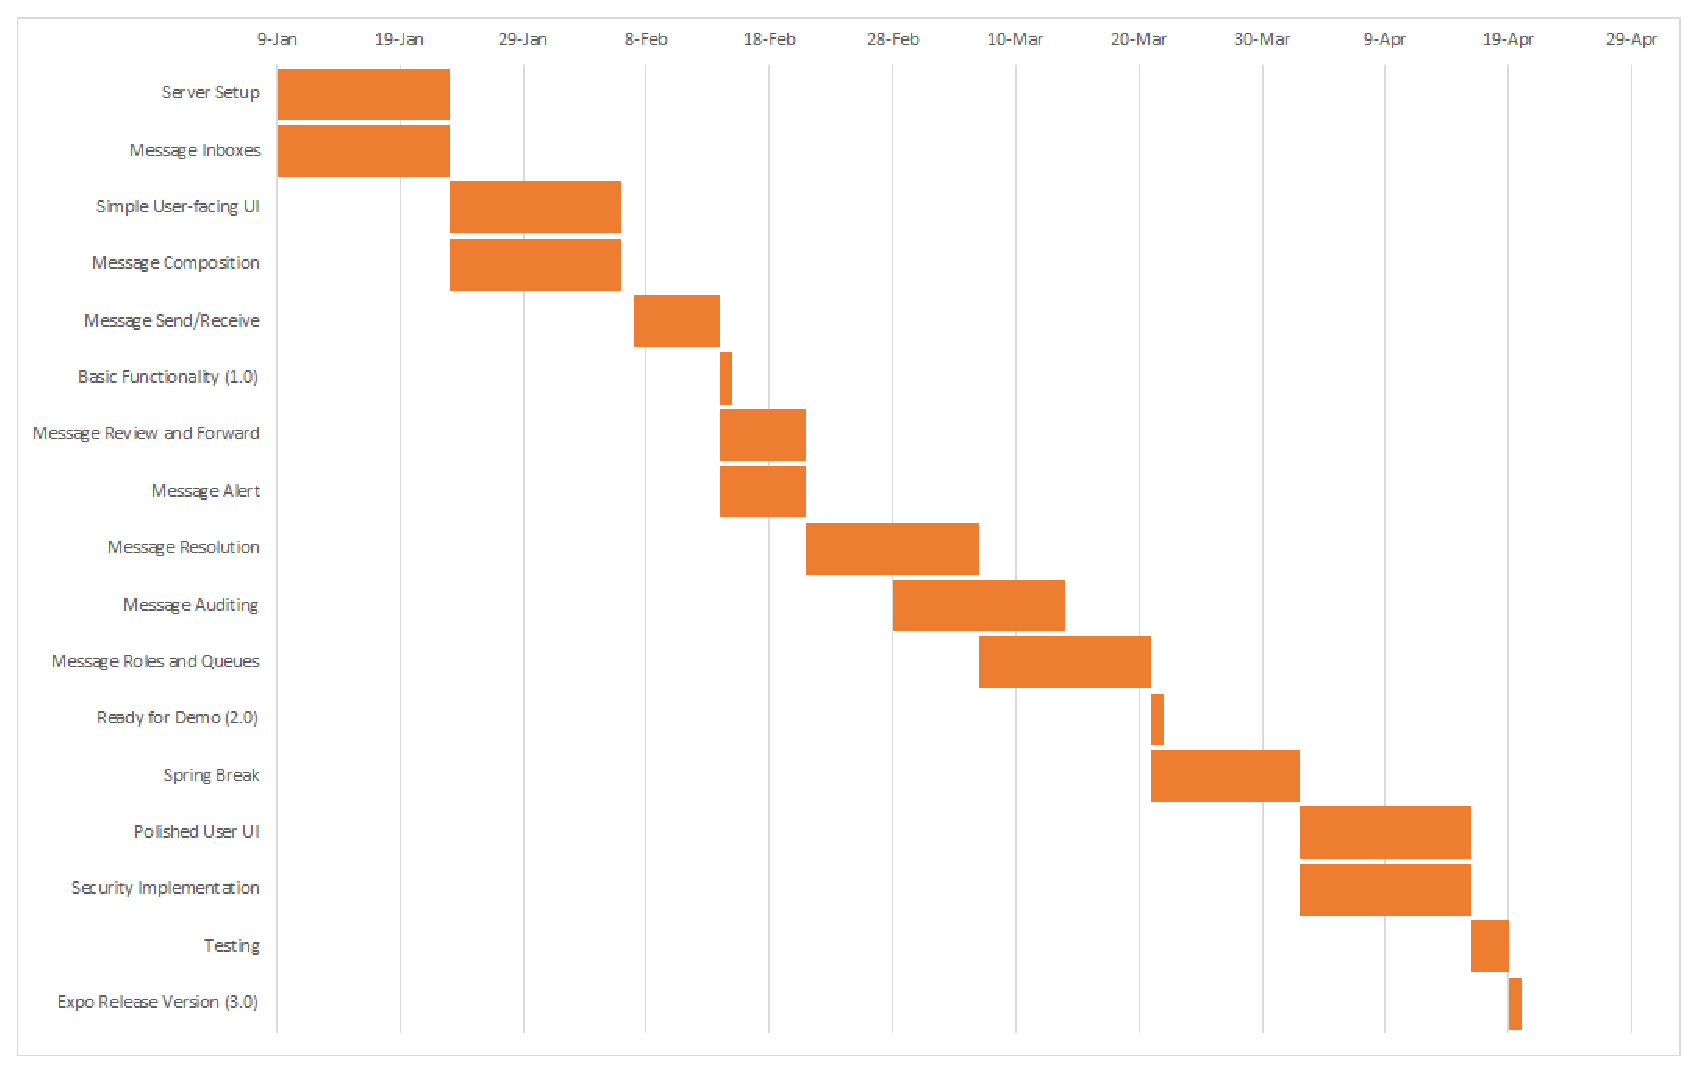
\includegraphics[origin=c,width=\textwidth,height=\textheight,keepaspectratio]{gantt-chart.eps}

\subsection{Changes}
As no more information about the VetHosp system was given to the development team, no integration with VetHosp was completed. In place of this the develpment team added an additional feature to allow messages to be exported to a PDF file that can then be uploaded into the VetHosp system. It was also decided that email notifications would be sufficient and sms messaging was not necessary.

\subsection{Final Gantt Chart}
\includegraphics[origin=c,width=\textwidth,height=\textheight,keepaspectratio]{final-gantt-chart.eps}

\newpage
\section{Design Document}

\subsection{Introduction}

\subsubsection{Purpose}
The purpose of this document is to layout a design plan for the ConnectBasket project. It will provide design viewpoints as well as identify stakeholders in the project. Each component's design will be explained in detail, and a timeline and testing information will also be provided for each component.
\subsubsection{Scope}
The ConnectBasket project is intended to be a stand-alone solution to help the Oregon State Veterinary Hospital increase the efficiency of communication between employees within the hospital and to patients. The hospital's current system is heavily paper based and error-prone, and this project will allow for a more efficient workflow.

Employees of the hospital will need to be able to enter messages about or connected to patients, route the message to other employees to take some action or add a note, and close the message as being completed. A notification system will be implemented to let employees know when they have a message to look at. There will also be a way for administrators to view a history of messages and their corresponding notes. This project will help the hospital quickly respond to patient inquiries and either answer their questions or schedule an appointment.

\subsubsection{Intended Audience}
The intended audience for this document is the Capstone development team working on the project as well as the client for the project. It is a plan for how the Capstone development team will implement the project. In addition to that, it will provide the client with information about the design and timeline for the development of the project.

\subsubsection{Stakeholders}
The stakeholders in this project include the client and the employees of the hospital. The client is working with both the Capstone development team and the hospital to complete the project. He will not be directly involved in using the product once it is developed. The employees of the hospital will be the end users of the project and interact with the finished product as a part of their daily jobs.

\subsubsection{Glossary of Terms}
Capstone - CS 461 class at Oregon State that the developers of ConnectBasket are in \newline
Capstone development team - The developers of ConnectBasket\newline
ConnectBasket - A web application being created for the OSU Veterinary Hospital\newline
Hospital - Referring to the OSU Veterinary Hospital\newline
Message - Initial information taken down by a receptionist\newline
Mobile Devices - Smartphones or tablets\newline
Note - Information added to a message at some point before the message is closed by a user the message was routed to\newline
OSU - Oregon State University\newline
Owner - A person who owns a pet that is a client of the hospital\newline
Patient - An animal who has/is going to be treated at the hospital \newline
Route - Send or transfer, usually referring to the forwarding of a message to one or more staff members\newline
VetHosp - The hospital management system used by the OSU Veterinary Hospital for keeping patient and owner records\newline
Vet techs - Veterinary technicians

\subsection{Design Viewpoints}

\subsubsection{Functional Viewpoint}

\paragraph{Functional Elements}
There are many functional elements that will make up the ConnectBasket web application. The four main pages of the web application are message entry, adding notes to messages, message viewing, and an audit trail of messages. The other functional element of the system is a database that stores the information collected through the application.

\begin{figure}[h!]
  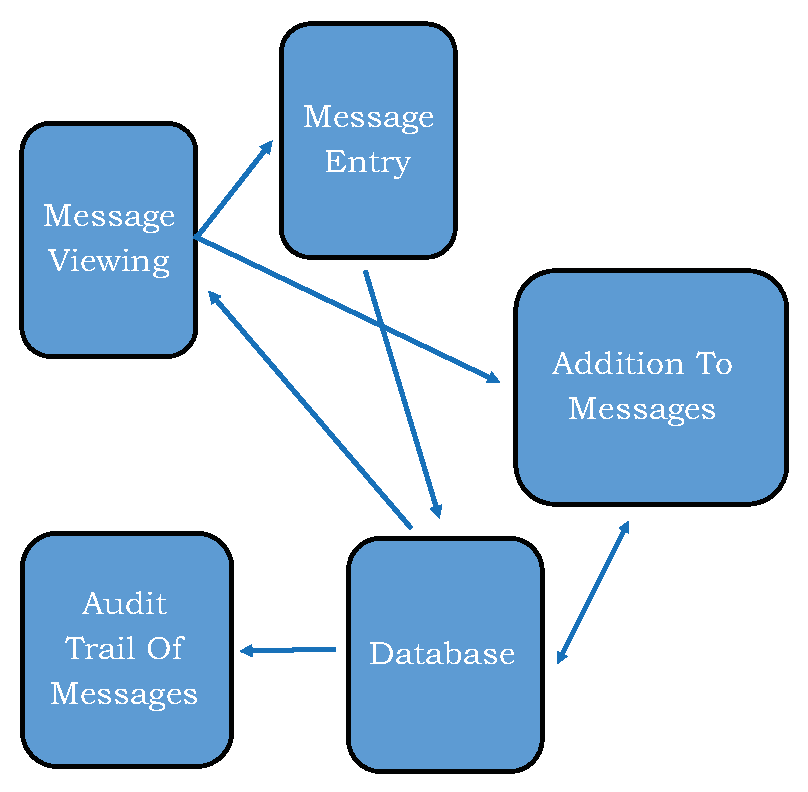
\includegraphics[width=0.5\textwidth]{functional_elements}
  \caption{Functional elements and their relationships}
\end{figure}

\paragraph{Responsibilities}
Each element has its own responsibilities. The message entry element will allow users to add a message to the database and route that message to other users. Adding notes to messages will allow users to add more information to a message that has already been created and either route to other users or close the message. Message viewing will allow users to see all messages that have been routed to them and see all of the previous notes that are associated with each message. The audit trail of messages will provide administrators with the ability to look at a history of messages and their notes that were created during a given time period. The database will have tables to store information about messages and their associated notes, and will have queries that return groups of messages that meet certain criteria.
\paragraph{Interfaces}
Each element will have its own page in the application. Message entry and adding notes to messages will be done through a web form, and the message viewing and audit trail of messages will be displayed through a table or grid. The database will be accessed through each page of the application. 

\paragraph{Primary Interactions}
Several of the pages will interact with each other. From the message viewing page, a user will be able to go to the message entry page or they will select a message and go to the adding notes to messages page for that message. Creating messages and adding notes to messages will insert new information into the database, where message viewing and audit logs of messages will pull information out of the database.

\subsubsection{Context Viewpoint}

\paragraph{Relationships and Interactions}
The ConnectBasket system has many relationships with its users. Users that work in reception and scheduling at the hospital will use the system to add new messages as well as view messages and their associated notes to call owners and give them answers to their questions or schedule appointments. Vet techs and doctors want to be able to view messages that have been routed to them and add notes to them. Administrators want to be able to view the audit logs of messages.

There will also be several external systems that ConnectBasket will interact with. A user profile framework will be used for managing users of the application and keeping login information secure. ConnectBasket will also interact with an email client in order to send notifications to users that a message is waiting for them. If proper access is provided to the development team, ConnectBasket will integrate with the VetHosp database to access patient and owner information.

\paragraph{Dependencies}
The notification feature of ConnectBasket will depend on users having access to their email through a mobile device or desktop computer that they check frequently. The user profile system will depend on users keeping their own information up to date in order to receive notifications and see their messages.

\subsubsection{Information Context}

\paragraph{Information Storage}
The information for ConnectBasket will be stored in a relational database. There will be tables that store information about messages, notes, owners, patients, and possibly users.  The different pages of the web application will allow for the information to be managed and displayed.

\begin{figure}[h!]
  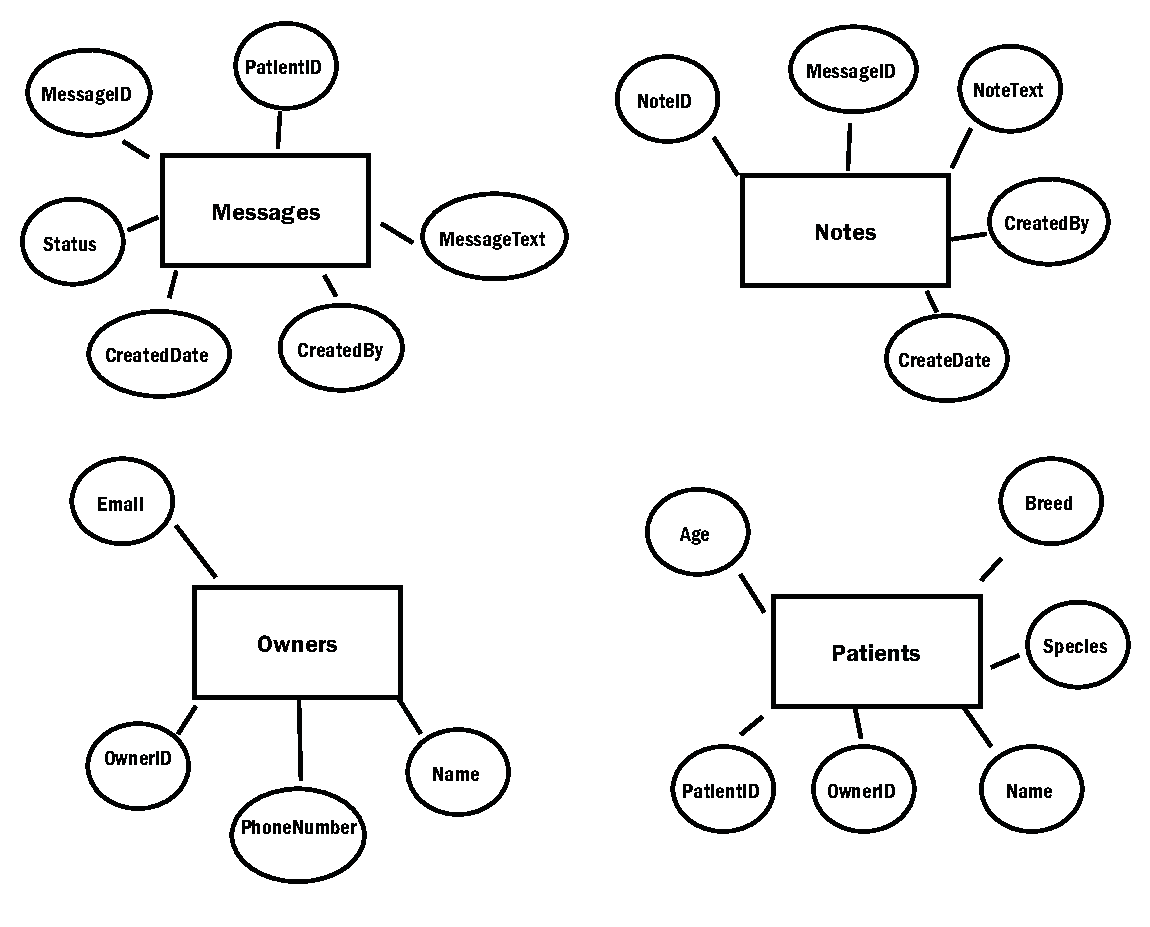
\includegraphics[width=0.5\textwidth]{database_design}
  \caption{Design of ConnectBasket database}
\end{figure}


\subsection{Components}

\subsubsection{Server Setup}

\paragraph{Details}
This project will require having a server configured to host the web application ConnectBasket. The application will not be supporting heavy traffic and does not have any specific speed requirements so the server requirements are not very strict.

The server will need to work with the web server software and database to make the application accessible to the users.  Users will interact with the server through the API created as a part of the ConnectBasket application.


\paragraph{Design Decisions}
The server operating system that will be used for this project is Linux Ubuntu Server. It was chosen for its low cost, short time to set up, and well written documentation. Most of the components of the project rely on the server being up and running so the decision was primarily based on the amount of time it will take to get set up \cite{ubuntu}.


\paragraph{Timeline}
The setup of the server will be the first priority in the development of this project. For this reason, the completion of this component will be done by the third week of winter term.

\paragraph{Testing}
There will be relatively little testing done for this particular component. If the web application is able to successfully be accessed, then this component will be considered successfully implemented.


\subsubsection{Web Server}

\paragraph{Details}
In order for ConnectBasket to work, the server must have web server software running on it. This software will allow users to access the web application running on the server from any mobile device or desktop computer that has internet access.

\paragraph{Design Decisions}
For this project, Apache HTTP will be the web server software that is used. It was chosen because of its cost, documentation, and flexibility. It is free software that can be used by the ConnectBasket development team for no cost. There is a large amount of well written documentation that will help during the setup period. Due to the short development window for the project, speed of implementation was a key factor in deciding which web server software to use. It is also a very flexible web server that can run on almost any hardware and with almost any server operating system\cite{apache}.


\paragraph{Timeline}
The web server software properly working is critical to the rest of the components being able to work and be tested. This component will be implemented as soon as the server component is completed. The web server software will be completely implemented by the end of week four of winter term.

\paragraph{Testing}
The testing of the web server software will be done by attempting to access the ConnectBasket application after it has been partially or fully created. This component will be considered complete when the web application is able to be used from all required devices.


\subsubsection{Database}

\paragraph{Details}
ConnectBasket will have a database that stores the information collected by the application. Messages that are created as well as all notes that are added to those messages will be stored in tables. There will also be tables that store information about the patients of the hospital and their owners. If the information is provided to the Capstone development team, the patient tables will be filled with information from the current VetHosp system. Otherwise, the tables will be filled with fake data for testing purposes, and patient information will have to be manually added by a hospital employee through ConnectBasket the first time an owner calls after the system is being used.

The data gathered through the application will be used for many different purposes. First, the messages entered and notes added will need to be immediately available through the web application for other users to view. Second, users will need to be able to see a chain of all notes that are associated with a certain message. Finally, administrators will be able to view an audit trail of all messages created and notes added over a given time period.


\paragraph{Design Decisions}
The database used for this project will be a MySQL database. It is important to have a relational database to store the data needed for the project. MySQL is also very flexible and can work well in almost any system. It is not the fastest database that could be used, but this application will not require any large amount of data manipulation, so the simple and easy to use interface provided by MySQL is the best choice\cite{mysql}.

\paragraph{Timeline}
The database will be critical for testing many other parts of the application, but will also be a large part of the project. Initial setup of the database and creation of tables will start around week two or three of winter term and finish by week five. The finished version week five is still subject to change, if the need for different or more tables or queries is found during the development of the rest of the project.


\paragraph{Testing}
The database will be tested in several ways. Queries will be run on their own to make sure that the correct data is being returned, in addition to using the web application to test and make sure data can be added and updated.

\subsubsection{Mobile Notification System}

\paragraph{Details}
ConnectBasket will have the ability to notify users. Users will have unique profiles that can contain information about them, including their email. This email will be used, according to user specifications, to alert them on their mobile device when a message is received or some other event designated as important by the user occurs. ConnectBasket will rely on the user's email application on their mobile device to deliver alerts and notifications. The body of this email will contain a link to the relevant page appropriate to view the specific event. The email body will also contain identifiers for any other users involved in the activity, along with a short description of the activity.


\paragraph{Design Decisions}
Rather than email, using SMS was an alternative option. However, due to the small scale of this project, paying for a VOIP service to handle SMS to most providers is unreasonable, especially with such few differences between them \cite{notifications}. While it is possible to use email to send a SMS message, it requires that one know the user's cell phone provider. In addition, messages sent in this method can be ugly and cluttered, possibly resulting in the user ignoring the message, or even suspecting it as spam. On top of this, SMS messages are generally for personal communication, and an automated message relayer may confuse the users. Because of all this, the Capstone development team decided against using SMS here. The ideal choice would be to use native notifications for mobile devices, but this is also an unreasonable option, as ConnectBasket will be a web application and will lack native mobile versions. Notifications through a mobile browser are technically possible, but will only take effect while the page is open on the user’s phone, which is likely to be very rare and is not a good solution. Sending emails from a service email or a “noreply” account is easier than both, free when done directly like this, can reach users even when they do not have ConnectBasket open, and easy to avoid confusion with custom body content and a more appropriate medium than texting for automated messages.


\paragraph{Timeline}
Notifications should be a more simple element to the project, and should not take longer than a week to develop and test completely. While a primitive version can be created ahead of time if needed, actual use-case testing will not be possible until user profiles and user messages exist to a certain degree. Notifications will need to make use of user information, at minimum a user's contact information and their identifying username. Notifications will also need to make use of a message sent to a user, requiring the message system to be implemented and to the point where it can send at least basic messages to specific users.


\paragraph{Testing}
Testing notifications should be very simple. Basic functionality can be tested immediately, by sending a dummy message to a specific email. If the basic function works, it will alert the email's owner on their mobile device, should the settings be enabled. Otherwise, testing will occur after both profiles and messages are implemented, with success criteria being: notification sent automatically, notification sent upon user receiving a message, notification sent using contact information from the user's profile, and user being able to navigate to the message via the notification. If all of these things are possible, this feature will be considered finished.


\subsubsection{User Profile Framework}


\paragraph{Details}
Users of the ConnectBasket software will be able to securely log in to accounts containing potentially confidential information. These accounts will be unique and linked to a single employee of the hospital, though not every employee of the hospital must have an account. These accounts will have identifying information, for both the ConnectBasket backend to use, and for other employees to use. The user accounts will have profiles that contain their information. User accounts will have the ability to be part of one or multiple groups, which can also contain other users. These groups will be used by the issue tracker system.


\paragraph{Design Decisions}
The focus for this feature is, rather than the functionality of the users, the security of the accounts and the ability to log in from various devices. Users will have profiles, but these profiles will not need to contain much more information than a username, an email, some settings, and a list of groups the user is a member of. Thus, since there is not a lot of user information, the PHP user login framework HUGE will be used, or at least referenced, for the user logins for ConnectBasket \cite{huge}. HUGE is a simple framework without many fancy features, perfect for use in ConnectBasket. Other options researched by the team, like Userfrosting, were also simple and easy to use, but generally had more functionality than needed, which could lead to confusion or compatibility issues \cite{userfrosting}.

\paragraph{Timeline}
Users should be one of the first things implemented in the system. While the message tracking functionality of ConnectBasket does not necessarily depend on users to exist, it is not functional and cannot be tested without it. Thus, user profile functionality is likely one of the first parts of the project software that should be done, once the web server is ready. It will need to be mostly implemented to allow other features to be started or tested.

\paragraph{Testing}
Testing a basic user login function is as simple as seeing if a login is possible. This can be tested early in the project, possibly even offline, before the web server is prepared on a developer’s personal computer. Once the webserver and database, a basic user-facing front-end is prepared, and user logins are implemented, they can be tested with success criteria being: a user can, without cookies in place, or in an “incognito mode”, or a new device, navigate to the ConnectBasket webpage and log in to their unique account using a username and password, a user can view information that the issue tracking system provides for them, a user cannot see messages unrelated to them, a user can change contact information, a user can log out, a different unique user can log in and do all of the above, and a user can close the browser or navigate to another page and be able to return to the ConnectBasket site without needing to log in again. All of these tests should also be verified on a mobile device as well.


\subsubsection{Issue Tracker Framework}

\paragraph{Details}
The core functionality of ConnectBasket is similar to many issue trackers or Kanban boards, without the graphical interface or “board” layout. ConnectBasket will include features one could expect from any issue tracker, but personalized for the hospital. The core of the issue tracking is the messages sent between users, which should be secure, accurate, and relatively fast. These messages will be directed to users and to groups. Users, as mentioned in the user profile framework section, can be part of groups, and can view and add notes to messages sent to these groups. These messages can be forwarded to other users or groups, or closed. These messages will have a history, which will contain and report the activity of a message, with all potentially relevant details. Messages will have multiple “states” such as closed, open, and duplicate that can be changed on demand.


\paragraph{Design Decisions}
Much of the desired functionality for this project is visible in the message system. Since much of what the client is asking for is similar to a ticketing system or kanban board, the development team will be looking for examples in similar technologies. The team considered simply wrapping an existing solution with a different user interaction system, but found that such a solution would contain too many unneeded features, and would not be much effort for a senior Capstone project. There are a few open source options that do similar or almost exactly what is requested by the client, but these are unlikely to fulfill the needs of this project for the reasons listed above and because the client has requested specific features that may not exist in these solutions. The team will be implementing an issue tracking message system from scratch, using the Best Practical Issue Tracker as a guide for what the final product may look like, and to use as reference should any roadblocks or issues be encountered \cite{bestpractical}.


\paragraph{Timeline}
This feature depends on the physical hardware and the webserver existing before implementation. While it cannot be formally tested beforehand, development can be done offline on a development computer. This work may not function in the same way as it will when on a webserver, so development will also need to take place on the server regardless of how much is done offline. This feature depends on and cannot be completed until the webserver has been implemented. In addition, to view any meaningful output and for testing, the user login feature will need to be implemented to some degree.


\paragraph{Testing}
A successful test of this feature denotes a working version of ConnectBasket. Early tests before full completion will likely be on whether or not the feature is capable of sending a message to a dummy user, and allowing users to enter and view messages.



\subsubsection{Content Delivery Network}

\paragraph{Details}
A content delivery network, or CDN, is a group of servers that are distributed geographically that work together to quickly deliver Internet content, such as images, videos, and HTML pages. Currently, most web traffic is served through CDNs, and CDN's can also help protect against some malicious attacks. Reasons to use a CDN include improving website load times, increasing content availability, and improving website security \cite{cdn}.


\paragraph{Design Decisions}
The CDN chosen for the ConnectBasket project is Cloudflare. The CDN that Cloudflare provides is designed to optimize security and performance, has multiple price levels, and is easy to set up. Cloudflare's CDN provides a flat price per month that does not depend on bandwidth, which makes it a good choice because there will never be any unexpected spikes in cost\cite{cloudflare}.


\paragraph{Timeline}
As this feature is not a required one for the project, its development will not be a priority. The addition of a CDN will be done after all other parts of the project are complete. This would likely be done in the final week of winter term or during spring term.


\paragraph{Testing}
The testing of the CDN would be minimal. The only testing that would need to be done is to make sure all features of the web application were still working after the CDN had been set up. As long as it does not cause problems with the functionality of ConnectBasket, it will be considered working.

\subsubsection{Web Development Framework}

\paragraph{Details}
A web development framework is considered to be tools and resources used by software developers to create and manage websites \cite{webdevframework}. Web development frameworks extend the capabilities of a language and provide libraries so developers do not have to start from scratch and hand-code everything \cite{framework}. ConnectBasket will have many basic features that most web development frameworks will provide libraries to easily implement. Using a web development framework to complete this project will help to speed up the development process and make the finish product aesthetically pleasing and user friendly.

\paragraph{Design Decisions}
The web development framework that will be used for the ConnectBasket web application is AngularJS. AngularJS was created and is maintained by Google and provides a powerful framework for building quick and easy to use web applications. It is a Javascript framework that extends basic HTML, adding many useful features that will work nicely to provide the features needed for ConnectBasket \cite{angular}. AngularJS was chosen for this project because it provides simple, easy to use tools that can build everything the project needs to have.


\paragraph{Timeline}
The web development framework will be used to create the ConnectBasket application. Development will begin at the start of winter term and will continue until the end of winter term and into spring term until the project is complete. Development can be done on the development team’s computers, but for full testing, the setup of the web server and database will need to be completed first.


\paragraph{Testing}
The testing of the ConnectBasket application created by the web development framework will need to be very thorough. There will need to be tests done of all of the individual features that make up the web application. In addition to testing by the developers, testing will need to be done with the users of the application to receive feedback and make final changes to the project.


\subsubsection{Software Design Pattern}

\paragraph{Details}
A design pattern is a solution to a general problem that can be reused in multiple situations. There are many different design patterns that can be used for a variety of situations, but often, there is one pattern that best fits a scenario.  


\paragraph{Design Decisions}
The design pattern that will be used for the ConnectBasket project is MVC, or Model-View-Controller. There are three components of MVC: Model, View, and Controller. The Model represents the data, the structure of the data, and how the data is represented in the application. The View is the component that makes the data displayable to the user in a useful way. The controller supplies an interface between the model and view components, taking the data from the model and converting it into something that can be used by the view component to display to the user \cite{mvc}. Using the MVC design pattern for the ConnectBasket project makes sense, because it can be split into these three components. The Model component will be the patient and owner data in the database. The View will be the interface of the application. The Controller will be the way that the Data and View components communicate and are connected. Additionally, there are three developers on the development team, which makes it easy to assign roles. 


\paragraph{Timeline}
The software design pattern is used throughout implementation of the project and will be finished when the project is complete during spring term. It is closely associated with the web development framework and they will be completed at the same time.


\paragraph{Testing}
The chosen design pattern will allow for easier testing of the finished ConnectBasket application through unit tests that can test each function that the Controller provides.


\subsection{Conclusion}

\subsubsection{Summary}
ConnectBasket is a web application that will be hosted on a server running a Linux Ubuntu Server operating system and an Apache HTTP web server. A custom database will be created for the project using MySQL. User notifications will be done through email and user profiles will be managed through a user profile framework. The web application will be developed using the AngularJS web development framework and create a customized system for managing hospital communications. The architecture of the application will follow an MVC software design pattern.

\subsection{Changes}
There were two main changes made to the initial design of the project. The first was not using an existing user profile framework. The development team decided to manage user profiles as a part of the ConnectBasket website in order to better provide the exact needs of the client. The second change was that no integration with VetHosp was done because the development team never received any additional information that would allow for that integration to be done.

\newpage
\section{Tech Review (Henry)}

\subsection{Introduction}

\subsubsection{Reason for Project}
The current software system used by the Oregon State University Veterinary Hospital for communication is out of date and inefficient. Their current process is very slow and manual, with lots of movement around a large hospital and unnecessary printing of papers. For instance, if an owner calls the hospital with a medical question, the receptionist would log the message into the computer, print it out, and physically walk the paper across the hospital to put in a spinning queue. When a doctor or other staff member looks at it, they would write an answer or necessary action on the paper, and physically carry the paper to the next location. Eventually, after it reaches all the necessary staff, it would be returned to the receptionist, who would then call the owner back to provide them with the information they requested, whether that is an answer to a question or to schedule an appointment. 

\subsubsection{Overview of Project}
This project aims to create a new stand-alone solution, ConnectBasket, that will streamline the communication process in the hospital. In this document, three main components of the project will be examined, looking at three different technologies for each that could be used to implement that component. ConnectBasket will be a web-based application, so it will be important to set up a server with the best operating system for this project. There will also need to be web server software that is compatable with the server operating system and meets all of the requirements of the project. Lastly, the information collected by the application will need to be stored in a database, so it is important for the best option to be used.

\subsection{Server Operating System}

\subsubsection{Overview}
For this project, there will need to be a server to host the web based services involved in the project. Because servers are mainly used to run applications and do not need to be interacted with frequently by non-technical users, server operating systems focus on the ability to manage resources with little attention being paid to a user interface. There are many different choices of operating systems that can run on a server and this section will analyze three different options and show that one will be the best fit for the project.

\subsubsection{Criteria}
The criteria that will be used to choose the best server operating system for this project will be the cost, difficulty of setup, available support, necessary downtime, and amount of maintenance needed. For this project using low cost or free technologies will contribute to keeping the overall budget low. There is a relatively small time window for development of the project, so a fast and easy installation is very important. It will also be important to have to have a low maintenance system that will continue to work after the development team is gone.

\subsubsection{Potential Choices}

\paragraph{Linux Ubuntu Server}
Ubuntu is a distribution of Linux that is very popular on desktop computers, but also has a server version that is growing in popularity. Unlike the very popular Red Hat Linux distribution, Ubuntu is free. Updates and maintenance of the code and security of Ubuntu are made by the global community as well as a paid development team. There is twenty four seven support available that can be very important if a quick response is needed to critical errors. Ubuntu is an easy system to setup with an installation that can be completed in as little as fifteen minutes. Like other versions of Linux, Ubuntu Server is very easy to maintain and rarely requires reboots, making it ideal for an application that requires very little downtime \cite{ubuntu}. 

\paragraph{Windows Server}
The Windows Server operating systems have been very popular with businesses since they first came out. Many tools are provided that will work very well with Windows Server, including Microsoft SQL Server and Internet Information Services. A large number of successful businesses use Windows Server, which means that there are many examples of how to use it as a part of a business. Windows Server is considered by many to be the best server operating system for mission-critical systems, meaning that there is very little downtime required when using Windows Server. Windows Server has built in tools to help improve power efficiency of the server that can help lower power consumption for a company. A virtualization platform is also included with Windows server which can allow for easily migrating the system from one physical machine to another or allowing users to remotely access applications and run them like they were locally installed \cite{windows}.

\paragraph{Solaris}
Solaris is a version of Unix that has been developed as a server operating system. Solaris was created by Sun and they are also responsible for supporting it. This makes Solaris a good operating system for a user who will need a lot of help in setting up their system. Solaris is based off of Unix, which is an operating system that has been around a long time and is trusted by many businesses. A problem with Solaris is that it will not run on many different hardware systems including most HP and IBM systems. Solaris is not free, although there is a version of Solaris that is more similar to Linux and can be optained for free with optional paid support \cite{solaris}.

\subsubsection{Discussion}
Unix, which Solaris is based off of, has been around a long time compared to Windows Server and Linux Ubuntu Server, but is not currently as popular as either of the other two. Linux Ubuntu Server is completely free with optional support packages that can be purchased, in contrast to Windows Server and Solaris which both cost money. All of the operating systems provide key features that make any server operating system useful such as security, support, easy setup. It might be slightly harder to get support when using a Linux system than the other two because Linux isn't owned by anyone.

\subsubsection{Conclusion}
The best server operating system to use for this project is Ubuntu Server. Solaris is not free and does not provide as many features as Windows Server or Ubuntu, so it is definitely not the right choice for this project. Windows Server might provide slightly more features than Ubuntu, but all the server will be used for is to host a simple web application, so things like allowing users to run desktop applications remotely are not important for this project. For all of the important features to this project like setup, support, downtime, and maintenance, Windows Server and Ubuntu are not that different and both would be good choices. The main difference is that Ubuntu is free, and for that reason, it is a better choice than Windows Server for this project.

\begin{table}[h!]
\centering
\begin{tabular}{ |l|l|l|l| } 
\hline
\textbf{Criteria} & \textbf{Ubuntu Server} & \textbf{Windows Server} & \textbf{Solaris} \\ \hline
Cost & Free & \$100+ & Free version available \\ \hline
Difficulty of setup & Very easy & Slightly difficult & Easy \\ \hline
Available support & 24 x 7 support available & Some support available & Sun provides support \\ \hline
Necessary downtime & Very little & Very little & Very little \\ \hline
Maintenance needed & Almost none & Some maintenance needed & Some maintenance needed \\ \hline
\end{tabular}
\end{table}

\subsection{Web Server Software}

\subsubsection{Overview}
Web server software is essential to running a website, and allows the content created by developers to be displayed to the end users through a web browser. There are many different options to use and it will be important for this project to have one that meets all of the needs of the project.
\subsubsection{Criteria}
The most important factors for this project are a web server software that is well documented and fast to setup, as well as cheap and able to run at fast speeds with relatively little downtime. With the short time period for development, it will be critical to have a web server that is up and running quickly. In addition, a low cost is another factor to consider for this project. The web application will be very important to daily operations of the hospital making small amounts of downtime another factor in evaluation.
\subsubsection{Potential Choices}

\paragraph{Apache HTTP}
The Apache Web Server is very powerful and provides many useful features to its users. It is an open source software, making it free to use and also gives users of this software the ability to modify its source code to meet their needs. Features include a control panel, customizable error messages, authentication schemes, Domain Name Service, Simple Mail Transfer Protocol, and File Transfer Protocol. Apache can run on almost any operating system including Windows, MacOS, Linux, and Unix. There is also support for many different programming languages, including PHP and Python, and the ability to have SSL and TSL encryption for websites \cite{apache}.

\paragraph{Cherokee}
Cherokee is a high performing web server that runs quickly and is easy to set up. It supports many other technologies, such as PHP and SSL encryption, and can be run of many different operating systems including Linux, Unix, and Windows. Cherokee also provides updates that do not require any downtime. Another important feature of Cherokee is that it provides an easy to use configuration interface called cherokee-admin. Cherokee is also free and has a an open source code base that can be modified by anyone who wants to make changes to adjust the system to meet their needs \cite{cherokee}.

\paragraph{NGINX}
NGINX is a system that has been optimized to handle a large number of simultaneous connections. It provides support for PHP and Python as well as email protocols like SMTP, POP3, and IMAP. It is a very fast system that maximizes hardware efficiency. NGINX mainly only supports Linux and Unix based systems, and has very little support for Windows and other operating systems. There is plenty of documentation explaining how to use NGINX and training to learn more about the system. This software is open source and free to use with an optional purchase that includes support \cite{nginx}.

\subsubsection{Discussion}
Apache HTTP and NGINX are both widely used web servers compared to Cherokee, which is a much less used product. All three are open source, available for free, and provide many of the same features and support. NGINX doesn't support very many operating systems compared to both Apache and Cherokee, which support almost any operating system.

\subsubsection{Conclusion}
For this project, the best choice of web server software is Apache. It provides all of the features that are necessary for the project, and can run on almost any operating system, where NGINX can not. Cherokee is also a good choice, but is not as widely used and does not have as much support or documentation as Apache.

\begin{table}[h!]
\centering
\begin{tabular}{ |l|l|l|l| } 
\hline
\textbf{Criteria} & \textbf{Apache HTTP} & \textbf{Cherokee} & \textbf{NGINX} \\ \hline
Cost & Free & Free & Free \\ \hline
Documentation & Very well documented & Some documentation & Well documented \\ \hline
Setup time & Fast & Very fast & Fast \\ \hline
Necessary downtime & Very little & Very little & Very little \\ \hline
\end{tabular}
\end{table}

\subsection{Database}

\subsubsection{Overview}
A database will be a very important part of this project. User information as well as information about patients will need to be stored in the database. The web application will rely heavily on interaction with the database to provide the features users will need.

\subsubsection{Criteria}
Important factors to consider when selecting a database for this project are the cost, speed, compatability with chosen operating systems and web servers, and ability to provide easy ways to report on the data it holds. As always it will be important to keep the cost of the project low. Users will need to enter information while on phone calls with owners of the patients, so speed will be important as they don't want to waste the time of the person on the phone. Reporting on the data collected will be very important for administrators to evaluate the success of the hospital and the new system.

\subsubsection{Potential Choices}

\paragraph{MySQL}
MySQL is an open source database management tool that provides many important features. MySQL is known for its excellent data security and is used by many popular websites, including Facebook and Twitter. It provides high performance and excellent scalability that gives it great speeds for any size system and allows it to only take up as much space as needed. MySQL comes with a guarantee of no downtime and can work with almost any operating system and web server \cite{mysql}.

\paragraph{SQLite}
SQLite is a relational database management system that is imbedded into the system that is using it. It is a file-based database that interacts directly with the system making it very fast and efficient. The system is easily portable because it is contained in a single file on the system. SQLite uses a slightly modified SQL that has only a few features removed. It does not provide any ability to manage different users access to the database like some other management systems might \cite{sqlite}.

\paragraph{Microsoft SQL Server}
Microsoft SQL Server is a very easy to use and powerful database management system. It provides integration with tools like SQL Server Management Studio and SQL Server Profiler that help users manage their database. There is a lot of support and documentation provided for SQL Server and it is much easier to learn and get help with than many other SQL based products. SQL server is a paid product and purchasing comes with support from Microsoft \cite{sqlserver}.

\subsubsection{Discussion}
SQLite is a slightly less feature rich product compared to MySQL and Microsoft SQL Server. All of these systems can work with many different operating systems and web servers. Microsoft SQL Server is a paid product, in contrast to MySQL and SQLite, which can both be used for free.

\subsubsection{Conclusion}
The best database management system for this project is MySQL. The speed of SQLite is better than the other two, but is not worth the tradeoff of lost functionality for this application. Microsoft SQL Server provides slightly more features, documentation, and support than MySQL, but they are not important enough to the project to offset the large cost difference between the two.

\begin{table}[h!]
\centering
\begin{tabular}{ |l|l|l|l| } 
\hline
\textbf{Criteria} & \textbf{MySQL} & \textbf{SQLite} & \textbf{Microsoft SQL Server} \\ \hline
Cost & Free & Free & Around \$1000 \\ \hline
Speed & Fast & Extremely fast & Fast \\ \hline
Reporting capability & Good & Average & Excellent \\ \hline
Compatability & Works with any system & Designed for smaller systems & Works best with other Microsoft products \\ \hline
\end{tabular}
\end{table}

\newpage
\section{Tech Review (Kailyn)}

\subsection{Introduction}

\subsubsection{Reason for Project}
The current software system used by the Oregon State University Veterinary Hospital for communication is outdated and inefficient. In their current system of receiving messages, if an owner calls the hospital with a medical question, the receptionist would log the message into the computer, print it out, and physically walk the paper across the hospital to put in a spinning queue. When a doctor or other staff member looks at it, they would write an answer or necessary action on the paper, and physically carry the paper to the next location. Eventually, after it reaches all the necessary staff, it would be returned to the receptionist, who would then call the owner back to provide them with the information they requested. Currently, their process is very slow and manual, with lots of movement around a large hospital and unnecessary printing of papers.

\subsubsection{Overview of Project}
The ConnectBasket project will be a stand-alone solution that will streamline the communication process in the hospital. A receptionist will be able to receive a call and create a new message. They can then assign a category to the message and route it to the necessary staff, who will be able to add notes and reroute it to more staff members. Staff will receive notifications, by email or text, when they have a message waiting to be viewed. Staff will have profiles where they can select their notification preferences, as well as which categories of messages they want to receive. When the message returns to the receptionist, they can call back the owner and inform them of the decisions or recommendations by the staff. The whole chain of where the message has traveled to and who has seen the message or added notes will be visible. This will help the hospital track specific metrics, such as response time to calls. 

\subsubsection{Overview of Document}
In this document, three components of the project will be examined, looking at three different technologies for each that could be used to implement that component. ConnectBasket will be a web-based application, and a content delivery network will be useful for delivering internet content, as well as improving load times and security. ConnectBasket will also require a web development framework. Finally, a software design pattern will be helpful for developing a simple, effective user interface. 


\subsection{Content Delivery Networks}

\subsubsection{Overview}
A content delivery network, or CDN, is a group of servers that are distributed geographically that work together to quickly deliver internet content, such as images, videos, and HTML pages. Currently, most web traffic is served through CDNs, and CDN's can also help protect against some malicious attacks. There are four main reasons to use a CDN: to improve website load times, to reduce bandwidth costs, to increase content availability, and to improve website security \cite{cdn}. 

\subsubsection{Criteria}
For this project, security is an important factor to consider. Since the ConnectBasket website will contain patient and owner information, it is important that the website is secure. Another essential factor to consider for the ConnectBasket project is price. It is critical for the cost to stay as low as possible, so choosing a free or low cost CDN is important to the project. In addition, fast and easy setup for the CDN would be beneficial, since there is a relatively small time frame for the development of ConnectBasket.


\subsubsection{Potential Choices}

\paragraph{Cloudflare}
The CDN that Cloudflare provides is designed to optimize security and performance, has multiple price levels, and is easy to set up. Cloudflare's CDN provides a flat price per month that does not depend on bandwidth. There are four pricing levels. The free version is for personal websites. The Pro version is twenty dollars per month for professional websites. The Business version is two hundred dollars per month for websites and businesses requiring advanced security and performance. Finally, the Enterprise version is for companies requiring enterprise-grade security and performance, and Cloudflare muse be contacted to determine a monthly price. In addition, setting up Cloudflare is easy, taking less than five minutes to set up a domain \cite{cloudflare}.

\paragraph{Akamai}
Akamai serves thirty percent of internet traffic, and it optimizes networks for content delivery \cite{akamaicdn}. Akamai's CDN has three components \cite{akamaicdn}. The Aura Edge Exchange allows operators to deliver video content to customers \cite{akamaicdn}. The Aura Control System is a set of tools that allows operators to manage components such as performance and CDN security \cite{akamaicdn}. Lastly, Akamai Federeation allows operators to work with the Akamai Intelligent Platform, which is a cloud-computing platform. Akamai does not provide pricing information on their website; they must be directly contacted to get a quote \cite{akamaicdn}.  

\paragraph{Amazon CloudFront}
The Amazon CloudFront CDN is built on the Amazon Web Service (AWS) infrastructure, with forty-four Availability zones in sixteen regions, and there are plans for further expansion. This large network provides high performance for customers all over the world. CloudFront is a highly secure CDN, and for no additional cost, all customers benefit from the protections of AWS Shield Standard. Amazon CloudFront is easily integrated and works best with other AWS services, such as Amazon Simple Storage Service and Amazon API Gateway. For pricing, there are no fixed fees or long term contracts; payment is only for the data transfer and requests used to deliver content to customers \cite{amazoncloudfront}.


\subsubsection{Discussion}
Cloudflare and Amazon seem to have opposite pricing systems. Cloudflare has a fixed pricing system, where the amount of traffic per month does not affect how much is paid. In contrast, for Amazon CloudFront has a variable pricing system, where payment is only for the amount of data transfer and requests. Akamai does not provide pricing information, and so a price comparison is not possible. All three have a high level of security, and so they would all be good choices for that factor.

\subsubsection{Conclusion}
The best CDN for this project is Cloudflare because it has a fixed cost, which means there will not be any spikes in cost in a given month. In addition, the amount of traffic to the ConnectBasket website is unknown, so a fixed cost is more reliable. Amazon CloudFront would be a good CDN, especially since it integrates well with other AWS services, but it seems to be the best choice only if other AWS services are being used, and we are not using other AWS services.

\begin{table}[h!]
\centering
\begin{tabular}{ |p{.2\linewidth}|p{.2\linewidth}|p{.2\linewidth}|p{.2\linewidth}| } 
\hline
\textbf{Criteria} & \textbf{Cloudflare} & \textbf{Akamai} & \textbf{Amazon CloudFront} \\ \hline
Cost & Fixed cost per month & Unknown & Variable cost per month \\ \hline
Difficulty of setup & Very easy, taking less than five minutes & Easy, with 24/7 support from Akamai & Easy when used with other AWS services\\ \hline
Security & Secure & Secure & Secure \\ \hline
\end{tabular}
\end{table}


\subsection{Web Development Frameworks}

\subsubsection{Overview}
A web development framework is considered to be tools and resources used by software developers to create and manage websites \cite{webdevframework}. Web development frameworks extend the capabilities of a language and provide libraries so developers do not have to start from scratch and hand-code everything. A framework may include libraries, APIs, security, and compilers, among other things \cite{framework}.

\subsubsection{Criteria}
One important criteria for this project for web development frameworks is that it needs to be easily scalable to many different devices and sizes of devices. This is important because the ConnectBasket website will need to be accessible from staff's desktop or laptop computers as well as a variety of smartphone devices. Another key factor is it needs to be simple as opposed to cluttered with a large number of features that will likely go unused. This project is relatively simple, and so tons of features are not necessary. Additionally, a framework that is flexible would be best. 

\subsubsection{Potential Choices}

\paragraph{ASP.NET} 
ASP.NET was created by Microsoft, and it is used to create interactive and data-driven web applications\cite{asp.net}. ASP.NET works with HTML to create dynamic web pages. One advantage of ASP.NET is that it provides built-in Windows authentication, so it is secure \cite{asp}. In addition, an ASP.NET application can be written in a variety of languages, including C\# and Visual Basic \cite{asp.net}. 

\paragraph{AngularJS}
AngularJS is a JavaScript based web application framework that is open source and currently maintained by Google \cite{angular}. It is fast for development and creates simple, dynamic websites \cite{angularjs}. AngularJS uses HTML as a template and extends HTML syntax to describe a website or application's components easily. AngularJS provides data binding capability to HTML, provides reusable components, and is unit testable, among many other features. In addition, AngularJS is available on all major browsers and smartphones. One disadvantage of AngularJS is that it is not secure, and so server side authentication is needed to keep an application secure \cite{angular}.

\paragraph{ReactJS}
ReactJS is a JavaScript library that makes it easy to build user interfaces by creating reusable UI components\cite{react}. ReactJS involves thinking about everything as a component \cite{react}. Advantages of ReactJS include that it can be used with other frameworks, and can be used on the client side or the server side \cite{react}. One major disadvantage of ReactJS is that other tools will need to be combined with React to get a complete set of tools that is required for development \cite{react}. 

\subsubsection{Discussion}
AngularJS and ReactJS are both JavaScript based, while ASP.NET is very flexible because it can be written in more than one language. AngularJS is useful because it is available on all major browsers and smartphones, but a downside is that it is not secure and would still require server side authentication. However, another component of the project is user authenication, so it is not required that the chosen web development framework contains secure authentication. In contrast, ASP.NET is secure and provides built-in Windows authentication. ReactJS would be reasonable for creating reusable components, but it would possibly require additional tools for successful development. AngularJS also can easily create reusable components.

\subsubsection{Conclusion}
AngularJS is the best web development framework for the ConnectBasket project. The main reason for choosing AngularJS is because it is designed to quickly produce dynamic and elegant websites. It is well-documented and maintained by Google, which makes it a sensible choice. Even though it does not have user authenication, that is something that can easily be implemented using another technology. 

\begin{table}[h!]
\centering
\begin{tabular}{ |p{.2\linewidth}|p{.2\linewidth}|p{.2\linewidth}|p{.2\linewidth}| } 
\hline
\textbf{Criteria} & \textbf{ASP.NET} & \textbf{AngularJS} & \textbf{ReactJS} \\ \hline
Flexibilty & Can be written in multiple languages & Works with all major browsers and smartphones & Works with all major browsers and smartphones \\ \hline
Complexity & Moderately complex & Simple & Simple\\ \hline
Integration with other tools & Works best with other Microsoft products & Easily integrates with other tools & Easily integrates with other tools \\ \hline
\end{tabular}
\end{table}

\subsection{Software Design Patterns}

\subsubsection{Overview}
Software design patterns are a important part of any software application. One very important feature of this project is to provide a user interface that will be accepted by users who are reluctant to change. This means how users are able to interact with the data is very important and modeling a system that closely reflects their current system in a more efficient way is critical.

\subsubsection{Criteria}
One major factor to consider when choosing a software design pattern for this project is how well the system will be able to model data in a way that our system needs it to. Users will be inputting data into the system, which must to be able to display that information to other users. Some data will be filtered for specific users, while some data will need to be displayed as an overall summary for other users.

\subsubsection{Potential Choices}

\paragraph{MVC}
MVC is a software design pattern for implementing a user interface. It separates an application into three parts known as the model, view, and controller. The model is the structure of the data in the application and how the data is represented in the application. View is the component that makes the data displayable to the user in a useful way. The controller supplies an interface between the model and view components, taking the data from the model and converting it into something that can be used by the view component to display to the user. MVC supports the development of multiple different views for one model so the same information can be displayed in multiple ways if that is important for the application. It is also a very fast development process because one person or team can develop the view component while another works on the controller and another works on the model. This design pattern requires multiple developers for it to work properly \cite{mvc}.

\paragraph{MVP}
MVP is a software design pattern that is based on similar concepts to the MVC design pattern. It separates an application into four different components that are responsible for determining how a user can interact with the system. Those components are the view, view interface, presenter, and model. The view is responsible for determining how the user will see the information displayed while the view interface connects the view to the presenter. The presenter connects the view to the model, which is responsible for the data that is displayed by the view. A view will usually only be connected to one presenter. Testing can be done easily with this design pattern because all interactions are done through an interface. Development is sped up by the fact that multiple programmers can split up the components and work on them separately \cite{mvp}.

\paragraph{MVVM}
MVVM is a software design pattern that is an extension of the MVC design pattern. MVVM has four components, which are model, view, controller, and view model. In the MVVM pattern, view models convert data from the model layer into something that is usable by the view layer, which keeps the code for controllers from growing too large. In MVVM, the controller no longer depends on the model, so it is much easier to test. Views are only used to present the data they are given. The view controller interacts with both the view model and view layers and the view model also interacts with the model \cite{mvvm}.

\subsubsection{Discussion}
MVVM and MVP are both similar to MVC, and provide some additional features compared to MVC. In contrast to the four components of MVVM and MVP, MVC only has three components which can make it a simpler and easier to use pattern. MVVM and MVP have an additional components which further modularizes the functionality of each component and makes it easier to test.

\subsubsection{Conclusion}
The best design pattern to use for this project is MVC. The user interface for this project will not be very complicated, so, while having additional components might improve testability, it will not be worth it for the increased complexity. Having three components also provides the option for dividing the components between the three person development team, with one team member working on each component.

\begin{table}[h!]
\centering
\begin{tabular}{ |p{.2\linewidth}|p{.2\linewidth}|p{.2\linewidth}|p{.2\linewidth}| } 
\hline
\textbf{Criteria} & \textbf{MVC} & \textbf{MVP} & \textbf{MVVM} \\ \hline
Components & Model, view, controller & View, view interface, presenter, model & Model, view, controller, view model \\ \hline
Number of components & 3 & 4 & 4 \\ \hline
\end{tabular}
\end{table}


\newpage
\section{Tech Review (Taylor)}

\subsection{Introduction}

\subsubsection{Purpose}
The purpose of this document is to give an overview of what parts of the ConnectBasket project Taylor Kirkpatrick will have responsibility over,
and analyze the technologies that may be used for each part. Each part will choose a specific technology that may be used in the final project, 
along with justification for why.


\subsubsection{Scope}
ConnectBasket will be a web based portal for the OSU Veterinary Hospital that will streamline the way messages are moved around the hospital and 
provide a better way to track the route that messages have taken. When an owner calls the hospital, receptionists will be able to type a message 
into the computer, assign it a category, and route it to the necessary staff members, which may be service specific vet techs, house officers, or 
faculty. Those staff members will be alerted, either by email or text, that they have a message waiting for them in ConnectBasket, and once viewed, 
notes can be added and the message can be re-routed to other staff members. After a message has been addressed by the necessary staff, the message 
can be closed preventing further notes or comments. The audit trail of when the message was created and closed will be visible, along with all the 
notes, timestamps of notes, and staff who added the notes.


\subsubsection{Definitions, Acronyms, and Abbreviations}
\begin{itemize}
\item Capstone - CS 461 class at Oregon State that the developers of ConnectBasket are in
 
\item OSU - Oregon State University

\item Hospital - referring to the OSU Veterinary Hospital

\item Owner - a person who owns a pet that is a client of the hospital

\item Patient - an animal who has/is going to be treated at the hospital 

\item VetHosp - the hospital management system used by the OSU Veterinary Hospital for keeping patient and owner records

\item Mobile Devices - smartphones or tablets

\item CPaaS  - Communications Platform as a Service
\end{itemize}
\subsubsection{References}
\begin{thebibliography}{8}
\bibitem{userfrosting}
"Userfrosting | Modern user management framework for PHP", \textit{Userfrosting.com}, 2017. [Online]. Available: https://www.userfrosting.com. [Accessed: 14- Nov- 2017].\\
\bibitem{huge}
 panique and others, HUGE, (2015), GitHub repository, https://github.com/panique/huge \\ 
\bibitem{asp}
 Microsoft, "Introduction to ASP.NET Identity", \textit{Docs.microsoft.com}, 2017. [Online]. Available: https://docs.microsoft.com/en-us/aspnet/identity/overview/getting-started/introduction-to-aspnet-identity. [Accessed: 14- Nov- 2017].\\
\bibitem{trello}
 Trello, "Trello", \textit{Trello.com}, 2017. [Online]. Available: https://trello.com/. [Accessed: 14- Nov- 2017].\\
\bibitem{bestpractical}
 Best Practical, "Request Tracker", \textit{Best Practical Solutions}, 2017. [Online]. Available: https://bestpractical.com/request-tracker. [Accessed: 14- Nov- 2017].\\
\bibitem{twilio}
 Twilio, "Communication APIs for SMS, Voice, Video and Authentication", \textit{Twilio.com}, 2017. [Online]. Available: https://www.twilio.com. [Accessed: 14- Nov- 2017].\\
\bibitem{nexmo}
 Nexmo, "Nexmo - APIs for SMS, Voice and Phone Verifications", \textit{Nexmo.com}, 2017. [Online]. Available: https://www.nexmo.com/. [Accessed: 14- Nov- 2017].\\
\bibitem{twilio v nexmo}
 M. Grech, "Twilio vs. Nexmo: The Head to Head Showdown for Developers | GetVoIP", \textit{Getvoip}, 2017. [Online]. Available: https://getvoip.com/blog/2017/01/05/twilio-vs-nexmo/. [Accessed: 14- Nov- 2017].\\
\end{thebibliography}
\subsubsection{Overview}
The rest of the document will contain three sections with an overview of the parts of the ConnectBasket project Taylor Kirkpatrick 
is responsible for. Each section will contain five subsections, three to analyze specific technologies, one to compare them, and one 
to state the chosen technology with project-specific reasoning.

% ----------------------------------------------------------------------------------------------------------

\subsection{User Logins/Profiles}
A feature highly anticipated by the client, users must have persistent, personalized states to distinguish them from other users when tasks are to be 
passed on. These user profiles must be private and secure, one to each user. Messages may be user-specific and carry information that is confidential 
or otherwise not to be made accessible to everyone, even within the company. This part specifies what framework or project will be built off of to 
create these users and their logins and profiles. Of note is the possible overlap this system may have with the issue tracking technology, as those are 
usually distributed as whole projects, including user logins. While we do expect to be using one of these frameworks, it may clash with what the issue tracker 
framework brings to the table.
\subsubsection{Userfrosting}
Userfrosting is a complete and easy to use framework for PHP. It depends on the PHP tool Composer and also makes use of Node.js and Bower for client-side packages.
The framework fully automates and handles persistent user sessions without requiring the dev team to handle sessions manually between many potentially dynamically updating 
pages. Userfrosting also adds easily customizable and rather nice looking user profile pages, allowing a dev to simply present some information to users under the conditions 
that they desire. In addition, this framework provides simple methods for a dev to create user roles for role based control, and assign users to them. Lastly, the framework 
allows the creation of a user administration page for user operations. This interface can be easily built for non-technical users, and ease the process of user administration 
for them.[1]
\subsubsection{HUGE}
HUGE is a PHP framework for doing simple user authentication. HUGE came about in a time when PHP was lacking many quality login solutions, and was built
primarily off of the password\_compat library once it was released. HUGE is no longer in active development, but has remained an excellent choice when facing 
up against many other PHP frameworks. HUGE makes use of the official PHP password hashing functions, with many other nice features that one would expect in a 
login framework like email account verification, form encryption, a "remember me" function, etc. HUGE also offers many other nice features like URL rewriting 
(masking possibly sensitive info), and supports user portraits already. HUGE requires PHP 5.5 or above, a MySQL database, a handful of PHP extentions, a few 
developer tools, and software for sending mail if desired.[2]
\subsubsection{ASP.NET Identity}
ASP.NET includes a relatively robust user login API for use in ASP.NET projects. As this project may be done in ASP.NET, this is something worth checking. As the web
became wider and demanded even better user management support, ASP.NET created the framework ASP.NET Identity to keep up with alternatives, offering full support with
other ASP.NET packages along with the expected features in a login framework. Playing well with other ASP.NET packages is not to be underestimated, however, as a project 
built in ASP.NET is sure to have numerous other packages. The framework does, of course, support simple login features, along with more advanced things like social media 
integration and a persistent "remember me" cookie login, and role based control.[3]
\subsubsection{Comparison}
At a first glance, it appears that ASP.NET Identity lacks features compared to the other two options, and this observation is correct. However, it does boast the reliability of
Microsoft's products, and development with it in Visual Studio would be easier than the other two. Between the other two, Userfrosting is much more hands-off than HUGE, and 
while doing less complex and error prone work is nice, it also restricts the freedom of the developers. HUGE and Userfrosting have very similar features available, but HUGE may 
even boast more features. However, HUGE was never really formally released as anything other than a simple open source framework. Identity and Userfrosting are both more formal 
projects, and may not be as bug prone.
\subsubsection{Selection}
The HUGE framework is the tentative winner in this category. It is a happy medium between the hands-off GUIs of Userfrosting and the mostly manual configuration of ASP.NET Identity.
HUGE has roughly the same number of features as the other two combined, is much better documented than both, and has many years of fellow users for support that Identity may
not have, and Userfrosting is unlikely to have. This victory comes with a caveat, however, as it is dependent on what language the software is in. Should the dev team be unable to
use PHP, or otherwise choose not to in favor of ASP.NET or something else, HUGE would be useless for the project. Of the three present here, however, it is the better of them, 
while the others provide options should other development decisions invalidate HUGE as an option.

% ----------------------------------------------------------------------------------------------------------

\subsection{Issue Tracker}
The primary goal of this project is, in essence, to create a create a custom issue tracker, personalized for the veterinary hospital. The bulk of the requested features
for this project are in tune with making a non-IT bug or feature tracker. The features requested are both standard issue tracker features and more specialized items as 
well. Thus, finding a framework or at least a simple, freely licensed issue tracker to build off of would simplify the development of the bulk of the features and reduce
room for error.
\subsubsection{Trello}
Trello is a popular kanban style scrum team management application. It is currently owned and maintained by Atlassian, who also own the similar software JIRA, which is more 
technical and is not free. Trello allows easy "whiteboard style" organization for tasks, and can easily be applied to non-technical uses. Trello also has a robust API available 
to the public, and is what the developers use for further work on the product, proving the power of the API. Trello's interface is easy to read and navigate, and interaction
is simple and intuitive. Trello also works with mobile devices, supporting most modern mobile browsers as well as desktop.[4]
\subsubsection{Request Tracker}
Request Tracker, made by Best Practical, is an issue tracker designed for general use, instead of technical users. Request tracker has a very clean interface, with simple messaging
and includes user login support by default. Request Tracker is an entirely open source project, and the community and developers seem to be quick to fix discovered bugs or issues. 
Request Tracker boasts email integration and allows users to interact fully with the system through email only, not even needing to open the application to resolve or interact with
tickets.[5]
\subsubsection{Manual Issue Tracking}
This option involves creating a bare-bones, incredibly simple request tracker in-house. This option would have exactly the features desired and would integrate the easiest with the 
rest of the project, with the caveat of taking a significant amount of time. However, when parts of the project are still unknown, this is guaranteed to be the most fluid option, 
as the development team can change or customize anything they want at any time. 
\subsubsection{Comparison}
Creating the request tracker manually is a very valid option, as a major problem some of the other issue trackers may have is the extent of the features they have that are mostly 
unneeded. Trello, while probably the most reliable and one of the easier options is especially guilty of this, as users would hardly benefit from the visual style of a board, and 
tickets being open and unsecured may prove to be problematic. Request Tracker is a good middle ground, as it is not bloated with unnecessary features, but does not require a custom
built system.
\subsubsection{Selection}
Request Tracker would be the ideal here. It contains almost exactly the features the client is looking for, and has bells and whistles that the users might appreciate without being 
overwhelmed by them. Trello is much too bulky, and the kanban style is not very applicable in this case. If Request Tracker can be integrated with what the client wishes, or built off 
of into a new application, this would give the users the most functionality while reducing the risk of human error and more bugs that would be inherent in manually creating the issue 
tracking.

% ----------------------------------------------------------------------------------------------------------

\subsection{Notifications}
The client has specifically requested smartphone notifications when notable activity takes place related to a specific user. Users should be able to be alerted to any activity 
related to their user profile or role on their smartphone, should they so wish. The client has not specified how this notification is to take place, and so could be up to which technology 
is chosen. The initial idea for notifications, though alternatives were considered, was using SMS, as it does not depend on wifi connection, and anyone with a functioning phone would 
have the ability to receive such a notification, even without a smart phone. Push notifications, while pretty and useful, could be impractical or impossible as the ConnectBasket software 
will be a web application rather than a native mobile application.
\subsubsection{Twilio}
The Twillio tool allows an application to send SMS messages regardless of provider to a user, among other phone related features such as programmable calls and call redundancy allowing
for more reliable calls and messaging. Twilio has a nice looking interface and easy to understand setup, and offers unique features like voice call support and robust 
message quality of life improvements like sticky sender and MMS support. Pricing for Twilio varies, and while they offer free API keys for limited use, many features even for small uses 
are not free.[6]
\subsubsection{Nexmo}
Nexmo, recently acquired by Vonage, boasts all of the features one could expect from a CPaaS tool. It allows a user to send messages through most providers and includes useful functions in
the API for number screening, allowing a service to catch spam or malicious numbers before devoting resources to them. Nexmo also offers a real-time chat function to interact with users 
should such a situation be desired. Nexmo benefits from the resources of their parent company, able to operate in 80 countries, supporting many popular chat systems, and offers free inbound texts.
Pricing is on a per-text basis, but does not contain a free trial for most features.[7]
\subsubsection{Manual Email}
This option forgoes the external tools and the use of SMS entirely. Most email providers allow for drafting and sending off a simple email to a target address. While this option would not 
directly solve the issue of mobile notifications, it could be used to take advantage of an existing feature most smartphones have, email notifications. Notifications could be delivered by the user's 
email application, giving the user more control over when or what notifications they would like to see, and also should be free. 
\subsubsection{Comparison}
Without the option of push notifications, which would be ideal, pricing and immediacy are the most important things. Twilio and Nexmo are rivals in the CPaaS industry, and have similar pricing plans that
compete with each other. However, neither of them are free for the purposes of this project, as both lock messaging tools behind a "pay per text" plan. Emailing is free and may likely even be easier 
than the other two to use, but lacks the immediacy that a SMS provides and also may not be received if the user lacks a wifi connection.[8]
\subsubsection{Selection}
Manual Emailing is probably the best choice here. While it is possible that the client or a member of the college would be willing to pay for either Twillio or Nexmo, the features they offer are overkill
for this project, and these notifications may not even be used by many of the users. Those that do, however, would likely not appreciate texts every time there is any activity on a ticket.


\newpage
\section{Weekly Blog Posts}

\subsection{Henry}

\subsection{Kailyn}

\subsection{Taylor}

\newpage
\section{Final Poster}

\includegraphics[origin=c,width=\textwidth,height=\textheight,keepaspectratio]{poster.eps}

\newpage
\section{Project Documentation}

\subsection{Important Contacts}
\begin{itemize}
\item Kevin McGrath (Capstone Instructor) - D.Kevin.McGrath@oregonstate.edu
\item Kirsten Winters (Capstone Instructor) - kirsten.winters@oregonstate.edu
\item Chinweike Eseonu (Project Client) - Chinweike.Eseonu@oregonstate.edu
\item Kelly Warner (Process Improvement Manager) - kelly.warner@oregonstate.edu
\item Todd Shechter (Director of IT for COE) - shechter@engr.orst.edu
\end{itemize}

\subsection{Important Links}
\begin{itemize}
\item Capstone webpage: http://eecs.oregonstate.edu/capstone/cs/capstone.cgi?home=1
\item ConnectBasket webpage: http://vm-cs462-g39.eecs.oregonstate.edu/
\item VSphere: https://vc-classes.engr.oregonstate.edu
\item OSU VPN instructions: https://oregonstate.teamdynamix.com/TDClient/KB/ArticleDet?ID=51154 
\end{itemize}

\subsection{Using the Site}

\subsubsection{Accessing the Site}
The site can be accessed at http://vm-cs462-g39.eecs.oregonstate.edu/ if the user is on an OSU network or is using a VPN. To access the administrative section of the site, the url is http://vm-cs462-g39.eecs.oregonstate.edu/phpmyadmin/ . Credentials to the site will be covered in a later section.

\subsubsection{Creating a User}
Any existing ConnectBasket user with administrator permissions can create a user by selecting the 'Create User' option in the 'Admin' group on the navigation bar at the top of the page. First name, last name, username, and password for the new user are all required. The new user should be able to log in shortly after the form is submitted.

\subsubsection{Creating a Message}
Any ConnectBasket user can create a message by selecting the large 'Add Message' button on the home page or the 'Add New Message' option in the 'Messages' group on the navigation bar at the top of the page. Patient name, owner name, case number, method of contact, call type, and message urgency are all added to the message if filled in on this screen. Selecting a call type may cause more entry fields to appear depending on the type. The space to enter the message body is below these options and textboxes. The message recipient is selected from the dropdown menu below the body, and is routed to a specific group. The message will be visible to everyone in that group.

\subsubsection{Viewing a Message}
Any ConnectBasket user can view an unclaimed message sent to a group they are part of. Messages can be viewed by selecting the large 'View Messages' button on the home page or the 'View Messages' option in the 'Messages' group on the navigation bar at the top of the page. The inbox page will show all unclaimed messages for all groups the user is part of on the bottom with claimed messages appearing above them.

Selecting 'Details' on an unclaimed message will show the user more information about the message and will allow them to export this message as a pdf or claim the message. Users cannot take action on a message without claiming it. 
	
After claiming a message or selecting 'Details' on a claimed message from the inbox page, a user will be able to take action on a message. They can add a note to the message and route it to a group just like a new message, or they can add a note and mark the message as complete. Both actions will remove the message from the user's inbox and either re-route it to a group or simply remove it.

All present and past messages can be viewed by all users. A user can select the 'History of Messages' option in the 'Messages' group on the navigation bar at the top of the page to view them. This allows a user to view all messages sorted by date and time, and review the contents, check the status, or export a pdf of the message. This is the only place to view messages after they are marked as complete. No action can be done to change the message information or the notes attached from this page.



\subsubsection{Editing User Settings}
Any ConnectBasket user can change their own account settings. The edit profile page can be viewed by selecting the large 'Edit Profile' button on the home page or the 'Edit Profile' option on the navigation bar at the top of the page. To change the user's email, select the edit button and make edits as desired. Email notifications can be selected as on or off. Users can enable and disable groups in the third section. A user can be part of any number of groups, and may change them at any time. A user will receive all messages routed to any of the groups they have selected here, and may claim any of them. For any of these changes to be saved, the 'Update' button at the bottom of the page must be selected.

\subsubsection{Audit Log}
Any ConnectBasket user with administrator permissions can view a log of all actions taken by other users by selecting the 'Audit Log' option in the 'Admin' group on the navigation bar at the top of the page. The table on this page will show more recent actions at the top. All actions taken by users on the site such as creating a message, reading a message, claiming a message, etc. will be viewable here.

\subsection{Technical Documentation}

\subsubsection{Accessing the Server}
ConnectBasket is a VM in OSU's network. The hostname is vm-cs462-g39.eecs.oregonstate.edu. This can be accessed through any ssh client such as PuTTY. To access this server or the site, you must be on one of OSU's networks. To access the server or site from outside one of these networks, a VPN must be set up and used on the computer that needs access. On the server, var/www/html/Capstone-2017-2018-Group-39/ is the path to the git repo.

\subsubsection{Making Changes}
Changes to the site should be made through git. Changes should first be made on a local computer, then pushed to the git repo. After proper review, changes can be pulled to the clone of the repo on the server at var/www/html/Capstone-2017-2018-Group-39/. All git commands on the server must be run with sudo. After the repo has been updated on the server, changes will be present on the site.

Changes to the database can be done on the server or using the phpMyAdmin UI. phpMyAdmin can be accessed at http://vm-cs462-g39.eecs.oregonstate.edu/phpmyadmin/ with all of the ConnectBasket data being present in the ConnectBasket database. Changes made on the server do not require sudo access, but do require database permissions. Changes can be made with this command structure: mysql -u databaseUsername -pdatabasePassword -e 'USE ConnectBasket; Query' note the lack of a space between the -p and the password.

\newpage
\section{Recommended Technical Resources for Learning More}
\subsection {Helpful Websites}
\begin{itemize}
\item https://docs.angularjs.org/guide/introduction
\item https://www.w3schools.com/
\item http://php.net/
\item https://dev.mysql.com/doc/
\end{itemize}

\newpage
\section{Conclusions and Reflections}

\subsection{Henry}

\subsubsection{What technical information did you learn?}

\subsubsection{What non-technical information did you learn?}

\subsubsection{What have you learned about project work?}

\subsubsection{What have you learned about project management?}

\subsubsection{What have you learned about working in teams?}

\subsubsection{If you could do it all over, what would you do differently?}

\subsection{Kailyn}

\subsubsection{What technical information did you learn?}

\subsubsection{What non-technical information did you learn?}

\subsubsection{What have you learned about project work?}

\subsubsection{What have you learned about project management?}

\subsubsection{What have you learned about working in teams?}

\subsubsection{If you could do it all over, what would you do differently?}

\subsection{Taylor}

\subsubsection{What technical information did you learn?}

\subsubsection{What non-technical information did you learn?}

\subsubsection{What have you learned about project work?}

\subsubsection{What have you learned about project management?}

\subsubsection{What have you learned about working in teams?}

\subsubsection{If you could do it all over, what would you do differently?}


\newpage
\section{Appendix 1: Essential Code Listings}

\newpage
\section{Appendix 2: Photos of Project}


\newpage
\nocite{*}
\bibliographystyle{ieeetr}
\bibliography{final_report}


\end{document}
